%%%%%%%%%%%%%%%%%%%%%%%%%%%%%%%%%%%%%%%%%%%%%%%%%%%%%%%%%%%%%%%%%%%%%%%%
%%
%%  The Fundamental Equations of Hydrodynamics and Ideal MHD
%%  for Astrophysical Flows
%%
%%  Originally written July 2024 by R. Fisher.
%%  Corrections and edits August 3, 2026 by Claude Opus.
%%
%%%%%%%%%%%%%%%%%%%%%%%%%%%%%%%%%%%%%%%%%%%%%%%%%%%%%%%%%%%%%%%%%%%%%%%%

%\documentclass[letterpaper,11pt]{article}
 \documentclass[notoc]{tufte-handout}
%\usepackage[margin=1in]{geometry}
\usepackage{microtype}
\usepackage[utf8]{inputenc}

\usepackage{amsfonts}
\usepackage{amsmath}
\usepackage{amssymb}
\usepackage{physics}
\usepackage{comment}
\usepackage{mathtools}
\usepackage{cancel}

\usepackage{enumerate}
\usepackage{enumitem}

\usepackage{booktabs}
\aboverulesep=0pt
\belowrulesep=0pt

\usepackage{array}
\usepackage{adjustbox}
\usepackage{multicol}

\usepackage{xcolor}
\usepackage{float}


\usepackage{graphicx}
%\usepackage[textwidth=2.5cm, textsize=small]{todonotes}

\setlength{\headheight}{24pt}
\addtolength{\topmargin}{-9pt}

\newcolumntype{L}[1]{>{\raggedright\arraybackslash}m{#1}}
\newcolumntype{C}[1]{>{\centering\arraybackslash}m{#1}}
\newcolumntype{R}[1]{>{\raggedleft\arraybackslash}m{#1}}

\usepackage{parskip}
\setlength{\parindent}{0pt}
\setlength{\parskip}{1em}


\renewcommand{\vec}[1]{\mathbf{#1}}

\newcommand{\del}{\vec{\nabla}}

\newcommand{\E}{\vec{E}}

\newcommand{\B}{\vec{B}}


\everymath{\displaystyle}

%\usepackage[colorlinks=true, linkcolor=blue]{hyperref}
\hypersetup{
  colorlinks = true,
  linkcolor = blue,      % color of internal links
  citecolor = blue,      % color of links to bibliography
  filecolor = magenta,   % color of file links
  urlcolor = blue,       % color of external links
}

\setcounter{secnumdepth}{2}


\title{The Fundamental Equations of Hydrodynamics and Ideal Magnetohydrodynamics for Astrophysical Flows}

\author[Prof. Robert Fisher]{Prof. Robert Fisher\thanks{The University of Massachusetts Dartmouth Department of Physics}\thanks{Heidelberg Institute for Theoretical Studies (HITS), Sabbatical 2023-24}}

\date{Originally written July 2024 by R. Fisher.\thanks{Corrections and edits August 3, 2026 by Claude Opus.}}


\begin{document}

\maketitle

\begin{abstract}
These notes present the fundamental equations of hydrodynamics and ideal magnetohydrodynamics (MHD) in the context of astrophysical flows. The equations are derived from conservation laws and provide a mathematical framework for numerical simulations of astrophysical systems, including stars, accretion disks, and the interstellar medium. The notes aim to serve as a concise introduction for students and researchers in the field of astrophysical fluid dynamics.
\end{abstract}

\newpage

\setcounter{tocdepth}{2}
\tableofcontents

\newpage


\section{Systems of Conservation Laws}

Modern astrophysical simulation methods are all grounded within a single classical framework of the governing partial differential equations of fluid mechanics and magnetohydrodynamics.

\iffalse
These governing equations can be expressed in a single compact and fully covariant equation for the relativistic stress-energy tensor $T_{\mu \nu} $ of a fluid:

\begin {equation}
\boxed {{\partial \over \partial x^{\mu} } T_{\mu \nu} = 0}
\end {equation}
%
Here $x^\mu$  includes both the time (0) and spatial ($i$ = 1 - 3) coordinates.

Given the material and energy contributions to the fluid (including rest mass and relativistic kinetic energy, electromagnetic energy, and so on) this single equation can be unpacked into equations for mass continuity, momentum conservation, and energy conservation in the non-relativistic limit, yielding the classical Navier-Stokes and Euler equations for viscid and inviscid fluids, respectively. This approach has a fundamental elegance, since it emphasizes that it is the time ${\partial / \partial x^0} = 0$ and space translation invariance ${\partial / \partial x^{i} }= 0$ of a system that generate the conservation laws and give rise to the fluid equations.
\fi

In the following, we will first undertake a systematic approach to the fluid equations, developing a physically-grounded intuition about the physics involved.

%We will then return to the supreme elegance of this relativistic formulation.

\subsection{Continuity Equation in 1D}

Assume mass density (mass/length) of a 1D system is  defined at each point in space along the $x$ axis. Write the total mass within $[x_a,x_b]$  at time $t$ as $M_{ab}(t)$

%\begin{enumerate}[label = \roman*.]
%\begin{enumerate}
%    \item
     \begin{equation}
        \int_{x_a}^{x_b} \rho ({x},t)~\mathrm{d}x = \text{Mass within }[x_a,x_b] \text{ at time }t \equiv M_{ab}(t)
    \end{equation}
%\end{enumerate}
%
 \marginnote{The  $\equiv$ symbol simply means an equivalence by definition. Here it is used to denote that this expression defines $M_{ab}(t)$.}

{\bf If} the system is {\bf flux-conservative}, then {\bf no mass is added or lost within the spatial interval $[x_a,x_b]$ apart from that mass which flows into or out of this region}, and we can write

\begin{align}
\frac{\mathrm{d}}{\mathrm{d}t }~\int_{x_a}^{x_b} \rho ({x},t)~\mathrm{d}x & = \frac{\mathrm{d}M_{ab}(t)}{\mathrm{d}t } \\
& = f(x_a,t) - f(x_b,t)
\end{align}
%
This last statement is not a definition but a physical assumption: it asserts that the only way mass changes inside the interval is by flowing across its two endpoints, and in so doing it {\it defines} the mass flux $f(x,t)$ at a point.\marginnote{Note that the signs are fixed by which way is ``in.'' Flux entering at the left endpoint $x_a$ adds mass; flux leaving at the right endpoint $x_b$ removes it.}

To find the {\bf total} change of mass in $[x_a,x_b]$ over a time interval, integrate this equation in time and apply the fundamental theorem of calculus:

\begin{equation}
\int_{t_1}^{t_2} \frac{\mathrm{d}}{\mathrm{d}t } \left[ \int_{x_a}^{x_b} \rho ({x},t)~\mathrm{d}x \right] ~\mathrm{d}t  = \int_{t_1}^{t_2} \left[ f(x_a,t) - f(x_b,t) \right]~\mathrm{d}t
\end {equation}

\begin {equation}
\hypertarget{star}{}\qquad \int_{x_a}^{x_b} \rho (x,t_2)~\mathrm{d}x - \int_{x_a}^{x_b} \rho (x,t_1)~\mathrm{d}x  =  \int_{t_1}^{t_2} \left[ f(x_a,t) - f(x_b,t) \right]~\mathrm{d}t \qquad (*)
\label{eqn:integral_form}
\end {equation}

%\begin {equation}
%M_{ab}(t_2) - M_{ab}(t_1) =   \int_{t_1}^{t_2} \left[ f(x_a,t) - f(x_b,t) \right]~\mathrm{d}t
%\end {equation}
%hypertarget{star}{(*)} %=  \int_{t_1}^{t_2} \left[ f(x_a,t) - f(x_b,t) \right]~\mathrm{d}t
%\end{align}

The left-hand side of this equation is the total change of the conserved mass within the interval  $[x_a,x_b]$, $M_{ab}(t_2) - M_{ab}(t_1)$. Note that the right-hand side of this equation represents the time-integrated flux around the boundary of the region  $[x_a,x_b]$. {\bf In other words,  one only needs to know the time-integrated fluxes over some time interval around a fixed boundary of a region to determine the change in the conserved quantity within the boundaries.}  As we will see, this seemingly trivial statement is in fact the foundational basis of all modern numerical methods for systems of conservation laws.

If $\rho (x, t)$ and $f (x, t)$ are $C^1$, and both anti-derivatives in space and time are defined (in the Riemann-integrable sense), then by the second fundamental  theorem of calculus (Newton--Leibniz):

\begin{align}
\rho(x,t_2) - \rho(x,t_1) & = \int_{t_1}^{t_2} \frac{\partial}{\partial t}\rho(x,t)~\mathrm{d}t \\
f(x_a,t) - f(x_b,t) & = -\int_{x_a}^{x_b}\frac{\partial}{\partial x}f(x,t)~\mathrm{d}x
\end{align}
%
\marginnote{Watch the minus sign in the second line. The fundamental theorem gives $f(x_b) - f(x_a) = \int_{x_a}^{x_b} \partial_x f~\mathrm{d}x$, and what appears on the right-hand side of $(*)$ is the {\it negative} of this, since it is the {\it inflow} that adds mass.}
Substituting both into $(*)$ and collecting everything under a single double integral,

\begin{equation}
\int_{t_1}^{t_2}\int_{x_a}^{x_b} \left[ \frac{\partial}{\partial t}\rho(x,t) + \frac{\partial}{\partial x}f(x,t)  \right]~\mathrm{d}x\mathrm{d}t = 0
\end{equation}

Because this equation holds for any $x_a$, $x_b$ and $t_1$ , $t_2$, the integrand must be identically zero. This last step is one we will use repeatedly, so it is worth isolating and naming once and for all:

\begin{center}
\fbox{
\begin{minipage}{0.90\linewidth}
{\bf Lemma (du Bois-Reymond).} If $h$ is continuous on a region $\Omega$ and $\int_{\omega} h ~\mathrm{d}\omega = 0$ for {\it every} subregion $\omega \subseteq \Omega$, then $h \equiv 0$ throughout $\Omega$.
\end{minipage}
}
\end{center}
%
The proof is very simple, and can be sketched out as follows. If the integrand is continuous ($C^0$) and {\it does not} identically vanish, then one can pick some neighborhood surrounding a point in which the integrand has the same sign, and therefore a non-zero integral, establishing the result by proof by contradiction.\footnote{See Lin \& Segel, ``Mathematics applied to deterministic problems in the natural sciences,'' \S 4.1. In the calculus of variations this same statement travels under the name of the {\it fundamental lemma}.} Applying the lemma,

\begin{equation}
    \frac{\partial}{\partial t}\rho(x,t) + \frac{\partial}{\partial x}f(x,t) = 0
\end{equation}

This is known as the continuity equation in physics.

\subsection{Hydrodynamical Equations in Multiple Dimensions}

In $D$ dimensions, we can generalize the arguments above to consider a $D$-dimensional volume rather than a line.  \marginnote{In $D$ dimensions, the mass density  has dimensions of mass per length$^D$, and flux is a vector $\vec {f}$ with dimensions of mass per time per length$^{D-1}$.} The total mass per unit time flowing {\it out} through the surface area $A$ bounding the region $V$ is simply the dot product of the mass flux with the surface area vector, so the rate of change of mass {\it within} $V$ is the negative of this quantity:


\begin{equation}
      \frac{d M}{d t}  =  - \oint_A  \vec {f} \cdot ~\mathrm{d}\vec {A} =  - \int_V  \del \cdot  \vec {f}  ~\mathrm{d} {V}
\end{equation}
%
Here, the second equality follows from the divergence theorem, again assuming that the flux $\vec {f}$ is sufficiently smooth that its divergence can be calculated.  Note that the negative sign arises because $\vec {f} \cdot ~\mathrm{d}\vec {A} > 0$ represents a mass outflux through the surface bounding the volume $V$.

The total mass contained in the volume $V$ is simply

\begin{equation}
     M =  \int_V  \rho ~\mathrm{d} {V}
\end{equation}

So the rate of change of the mass inside $V$  is simply

\begin{equation}
     \frac{d M}{d t} =  \frac{d}{d t} \int_V  \rho ~\mathrm{d} {V}   =  \int_V  {\partial \rho \over \partial t} ~\mathrm{d} {V}
\end{equation}
%
\marginnote{This step deserves a moment's care, and is the single most common place for confusion in this entire derivation. $V$ here is a region {\it fixed in space} -- an imaginary box we have drawn and left alone -- and not a co-moving blob of fluid. Because the limits of integration do not depend on time, the time derivative passes inside the integral and becomes a partial derivative. Had we instead chosen a volume co-moving with the fluid, we would have picked up additional terms from the motion of the boundary, and would need the Reynolds transport theorem. The fixed-volume, or {\it Eulerian}, point of view is the one that underlies grid-based simulation codes.}

Now we have two independent ways of writing $ d M /  dt$. These can be equated, and after application of the du Bois-Reymond lemma, yield the continuity equation in multiple dimensions:



\begin{equation}
    \frac{\partial}{\partial t} \rho(\vec{x},t) + \del\cdot \vec{f}(\vec{x},t) = 0
\end{equation}

If sources or sinks are present, they can be modeled by terms on the right hand side (``source terms''). Because the conservation law is a first-order partial differential equation, it admits discontinuous ``weak solutions'' which satisfy the integral form of the conservation law \hyperlink{star}{(*)}, and are not differentiable. Once the conservation law is {\it nonlinear} -- as the full system of Euler equations we are building toward certainly is -- these solutions may also no longer be unique, and an additional physical principle is required to select the correct one.\footnote{It is easy to understand why. We are typically interested in the inviscid Euler hydrodynamic equations, which formally admit both compressible shocks as well as their time-reversal, rarefaction shocks. Clearly, only the former are the correct limit as the viscosity approaches zero; the latter violate the second law of thermodynamics. It is worth stressing that such spurious solutions are generally not numerically {\it unstable} -- which is precisely what makes them dangerous. Roe's scheme without an entropy fix will converge perfectly happily to an entropy-violating expansion shock at a transonic rarefaction. The scheme is stable; the answer is simply wrong.} For example, shock fronts need an ``entropy condition'' to ensure uniqueness (see LeVeque, ``Numerical Methods for Conservation Laws,'' \S 3.8 for a short overview, and Reed \& Simon, ``Methods of Modern Mathematical Physics I: Functional Analysis'' \S V.4 for a more rigorous introduction).

For mass continuity, $\vec{f} (x,t)=\rho (x,t) \vec{v}(x,t)$, so we obtain our first fundamental fluid equation:
\begin{equation}
\boxed {\frac{\partial \rho}{\partial t} + \del\cdot (\rho\vec{v}) = 0}
\label {eqn:continuity}
\end{equation}
%
Note that for clarity, we have dropped the functional dependence on position and time. From here forward, and in the literature in general, the spatial and time dependence of the state quantities is generally assumed (eg, $\rho$ in place of $\rho (x, t)$).

Next, let's consider both momentum conservation and energy conservation. We can, for example, write the total momentum $\vec {p}$ within some volume $V$ as the volume integral of the momentum density $\rho \vec {v}$:

\begin{equation}
\vec{p} = \int_V \rho \vec{v}~\mathrm{d}V
\end{equation}

The rate at which $i$-momentum is carried out of the volume $V$ by the flow across its boundary is then
\begin{equation}
    \left( \dot{\vec{p}}_{\rm flux} \right)_i = \oint_S \rho v_i \sum_j v_j~\mathrm{d}S_j
\end{equation}
%
Note that frequently in physics texts, terms with repeated indices are assumed to be summations over these indices (as with $j$ here) according to the convention called Einstein summation notation. For clarity we will include the summations explicitly. Note also that $i$ here labels the {\it component of momentum} being transported, whereas $j$ labels the {\it direction of transport}; they must be kept distinct. \marginnote{Here $\mathrm{d}S_j$ denotes the $j$-th Cartesian component of the outward vector surface element $\mathrm{d}\vec{S}$, so that $\sum_j v_j \mathrm{d}S_j = \vec{v} \cdot \mathrm{d}\vec{S}$.}

Next, let's decompose the force acting on this fluid element into force per unit volume (body force) and surface force per unit area.

\begin{equation}
    F_{i}^{\rm tot} = \int_V F_{v,i}~\mathrm{d}V + \oint_S \sum_j \sigma_{ij}~\mathrm{d}S_j
\end{equation}
%
Here $F_{i}^{\rm tot}$ is the total $i$-component of the force acting on the fluid within $V$, and $F_{v,i}$ is the body force {\it per unit volume} -- gravity, in every application we will care about.

$\sigma_{ij}$ is the \textit{stress tensor}. Pascal's law tells us that for a fluid at rest -- or, equivalently, for an inviscid fluid, which supports no shear -- $\sigma_{ij}$ should be {\it isotropic}, with the form for an ideal (zero viscosity, zero conductivity) fluid:

\begin{align}
\text{stress } T_i(\vec{x},\hat{n}) & = \sum_j\sigma_{ij}n_j , \qquad \text{where} \quad \sigma_{ij} = -p\,\delta_{ij} = \begin{pmatrix}
    -p & 0 & 0 \\
    0 & -p & 0 \\
    0 & 0 & -p
\end{pmatrix} \\
\Longrightarrow \quad \vec{T}(\vec{x},\hat{n}) & = -p\,\hat{n}
\end{align}
%
In other words, the surface force on any element of area is directed along the inward normal, with magnitude $p$, irrespective of how that surface is oriented. It is worth being careful about {\it why} this form survives a change of coordinates. It is not because the trace of a tensor is invariant -- that is true but insufficient, since a tensor may have an invariant trace and still acquire off-diagonal components under rotation. The correct reason is that $\delta_{ij}$ is the unique rank-2 {\it isotropic} tensor, satisfying $\sum_{k,l} R_{ik}R_{jl}\delta_{kl} = \delta_{ij}$ for every rotation matrix $R$. Consequently $\sigma_{ij} = -p\,\delta_{ij}$ retains precisely the same diagonal form in every Cartesian frame.\marginnote{A real fluid has $\sigma_{ij} = -p\,\delta_{ij} + \tau_{ij}$, where the viscous stress $\tau_{ij} = \mu \left(\partial_i v_j + \partial_j v_i - \frac{2}{3}\delta_{ij} \del \cdot \vec{v} \right) + \zeta \delta_{ij} \del \cdot \vec{v}$ carries the shear and bulk viscosities $\mu$ and $\zeta$. Retaining $\tau_{ij}$ gives the Navier-Stokes equations; the word {\it ideal} throughout these notes means precisely that we set $\tau_{ij} = 0$.}

Writing this out, and equating the rate of change of momentum within $V$ plus the rate at which momentum is fluxed out of $V$ to the total force acting on $V$,

\begin{equation}
\int_V \frac{\partial(\rho {v}_i)}{\partial t}~\mathrm{d}V + \oint_S \rho v_i \sum_j v_j~\mathrm{d}S_j = \int_V F_{v,i}~\mathrm{d}V + \oint_S \sum_j \sigma_{ij}~\mathrm{d}S_j
\end{equation}

The divergence theorem applied to the surface integrals, along with the stress tensor $\sigma_{ij}=-p\delta_{ij}$ for an ideal fluid then yields:

\begin{equation}
\int_V \left[ \frac{\partial(\rho {v}_i)}{\partial t} + \sum_j \frac{\partial(\rho {v}_iv_j)}{\partial x_j} \right]\mathrm{d}V = \int_V \left[ F_{v,i} + \sum_j \frac{\partial \sigma_{ij}}{\partial x_j} \right]\mathrm{d}V
\end{equation}

Or, rearranging terms,

\begin{equation}
\int_V \left[ \frac{\partial(\rho {v}_i)}{\partial t} + \sum_j \frac{\partial(\rho {v}_iv_j)}{\partial x_j} - F_{v,i} - \sum_j \frac{\partial \sigma_{ij}}{\partial x_j} \right]\mathrm{d}V    = 0
\end{equation}

Because this result applies to any volume $V$, the du Bois-Reymond lemma implies that the integrand must be zero, which gives

\begin{equation}
\frac{\partial(\rho {v}_i)}{\partial t} + \sum_j \left (  \frac{\partial(\rho {v}_i {v}_j)}{\partial x_j} + \frac{\partial p}{\partial x_j} \delta_{ij} \right) = F_{v,i}
\end{equation}

The momentum equation can then be recast into conservative form, including the divergence of the momentum flux density tensor $\Pi_{ij}$ and the remaining body force $F_{v,i}$ as a source term:
\begin{equation}
\boxed {\frac{\partial(\rho {v}_i)}{\partial t} + \sum_j \frac{\partial \Pi_{ij}} {\partial x_j} = F_{v,i} }
\label{eqn:momentum_equation}
\end{equation}
%
The momentum flux density tensor $\Pi_{ij}$ is then seen to be $\Pi_{ij} = p \delta_{ij} + \rho v_i v_j$.

{\bf Energy conservation.}
Energy conservation for a fluid in a gravitational field produces a very similar result, and it is worth carrying the derivation through rather than simply quoting it, since the appearance of the pressure inside the flux is a genuine subtlety. Define the total hydrodynamic energy density $\rho E = \rho \epsilon_{\text{int}} + \frac{1}{2}\rho v^2$, where $\epsilon_{\text{int}}$ is the specific internal energy (internal energy per unit mass).\marginnote{Note that $\rho E$ deliberately does {\it not} include the gravitational potential energy. The gravitational contribution enters instead as the source term on the right-hand side.} There are exactly three ways the energy inside a fixed volume $V$ can change: it can be advected across the boundary with the flow, the surrounding fluid can do work on the boundary through the pressure, and the body force can do work throughout the interior.

\begin{equation}
\int_V \frac{\partial (\rho E)}{\partial t}~\mathrm{d}V = \underbrace{- \oint_S \rho E \sum_j v_j ~\mathrm{d}S_j}_{\text{advection}} \underbrace{- \oint_S p \sum_j v_j ~\mathrm{d}S_j}_{\text{pressure work}} + \underbrace{\int_V \sum_i F_{v,i} v_i ~\mathrm{d}V}_{\text{body force work}}
\end{equation}
%
The pressure work term follows directly from the stress we found above: the rate at which the exterior fluid does work on the material inside $V$ is $\oint_S \sum_i T_i v_i ~\mathrm{d}S = -\oint_S p \, \vec{v} \cdot \mathrm{d}\vec{S}$, which is negative when the fluid is expanding outward, exactly as the familiar $p \, dV$ work of thermodynamics requires. Applying the divergence theorem to both surface integrals and invoking the du Bois-Reymond lemma once more,

\begin{equation}
\boxed {\frac{\partial (\rho E)}{\partial t} + \sum_i  \frac{\partial \left[ (\rho E + p)v_i \right]}{\partial x_i} = \sum_i F_{v,i}  v_i }
\label {eqn:energy_equation}
\end{equation}
%
Note that it is the {\it enthalpy} density $\rho E + p$, and not the energy density alone, that is transported. With body force source term $F_{v,i} = \rho g_i$:

\begin{equation}
{\frac{\partial (\rho E)}{\partial t} + \sum_i  \frac{\partial \left[ (\rho E + p)v_i \right]}{\partial x_i} = \sum_i  \rho g_i v_i }
%\label {eqn:energy_equation}
\end{equation}
%
We have assumed throughout that there is no heat conduction, no radiative heating or cooling, and no viscous dissipation; each of these would contribute an additional flux or source term on the right.

\subsection{Primitive Form and the Lagrangian Derivative}

The three boxed equations above are written in {\it conservative} form: each has the structure $\partial_t (\text{density}) + \del \cdot (\text{flux}) = \text{source}$. This is the form a simulation code wants, for exactly the reason established in \S 1.1 -- it is the differential shadow of a statement about fluxes through boundaries, and it therefore continues to make sense across a shock, where the derivatives themselves do not.

Most students meet the fluid equations first in a different, {\it primitive} or {\it Lagrangian} form, and it is worth connecting the two. Define the {\it Lagrangian}, {\it material}, or {\it convective} derivative

\begin{equation}
\frac{D}{Dt} \equiv \frac{\partial}{\partial t} + \sum_j v_j \frac{\partial}{\partial x_j} = \frac{\partial}{\partial t} + \vec{v}\cdot\del
\label{eqn:lagrangian_derivative}
\end{equation}
%
which is the rate of change measured by an observer drifting along with the fluid, rather than one standing still at a fixed point in space. Expanding the conservative momentum equation with the product rule,

\begin{align}
\frac{\partial(\rho v_i)}{\partial t} + \sum_j \frac{\partial (\rho v_i v_j)}{\partial x_j} & = \rho \left( \frac{\partial v_i}{\partial t} + \sum_j v_j \frac{\partial v_i}{\partial x_j} \right) + v_i \underbrace{\left[ \frac{\partial \rho}{\partial t} + \del\cdot(\rho\vec{v}) \right]}_{= \; 0 \; \text{by continuity}} = \rho \frac{D v_i}{Dt}
\end{align}
%
so that Equations \ref{eqn:continuity} and \ref{eqn:momentum_equation} become simply

\begin{equation}
\boxed{ \frac{D\rho}{Dt} = - \rho \, \del\cdot\vec{v} , \qquad \rho \frac{D\vec{v}}{Dt} = -\del p + \rho \vec{g} }
\end{equation}
%
The second of these is Euler's equation, and it is nothing more than $m\vec{a} = \vec{F}$ applied to a parcel of fluid. The first says that the density of a parcel changes only if the flow is compressing or expanding it. \marginnote{The two forms are mathematically equivalent {\it only for smooth flows}. Across a shock the manipulation above requires derivatives that do not exist, and it is the conservative form that remains valid and that yields the correct Rankine-Hugoniot jump conditions. This is why essentially every modern astrophysical hydrodynamics code evolves the conservative variables $(\rho, \rho\vec{v}, \rho E)$ even though the primitive variables $(\rho, \vec{v}, p)$ are more physically transparent -- and why the conversion between the two sets is performed at every timestep.}

\subsection{The Poisson Equation}

The hydrodynamical equations utilize the gravitational acceleration $\vec {g}= -\del \Phi$, where $\Phi$ is the gravitational potential. The gravitational acceleration may sometimes be taken to be a spatial constant independent of location, for example in a planetary or stellar atmosphere. However, in a general self-gravitating system, the gravitational acceleration depends on all other masses, which are moving in time, and one must obtain the gravitational acceleration self-consistently.

To derive Poisson's equation in 3D, we start with Gauss's law for gravity, which states that the flux of the gravitational field $\mathbf{g}$ through a closed surface is proportional to the enclosed mass $M$. Mathematically, this is expressed as:

\begin{equation}
\oint_S \mathbf{g} \cdot \mathrm{d}\mathbf{A} = -4 \pi G M
\end{equation}
%
where $\mathrm{d}\mathbf{A}$ is the differential area element on the closed surface $S$, and $G$ is the gravitational constant.

Substituting $\mathbf{g} = -\del \Phi$ into Gauss's law:

\begin{equation}
\oint_S \del \Phi \cdot \mathrm{d}\mathbf{A} = 4 \pi G M
\end{equation}

We apply the divergence theorem, which relates the flux of a vector field through a closed surface to the volume integral of the divergence of the field over the region enclosed by the surface:

\begin{equation}
\oint_S \mathbf{F} \cdot \mathrm{d}\mathbf{A} = \int_V \del \cdot \mathbf{F} \, \mathrm{d}V
\end{equation}

Applying the divergence theorem to our expression:

\begin{equation}
\oint_S \del \Phi \cdot \mathrm{d}\mathbf{A} = \int_V \del \cdot \del \Phi \, \mathrm{d}V
\end{equation}

The term $\del \cdot \del \Phi$ is the Laplacian of $\Phi$, denoted by $\del^2 \Phi$:

\begin{equation}
\int_V \del^2 \Phi \, \mathrm{d}V = 4 \pi G M
\end{equation}

The mass $M$ within volume $V$ can be expressed in terms of the mass density $\rho$:

\begin{equation}
M = \int_V \rho \, \mathrm{d}V
\end{equation}

Substituting $M$ into the volume integral:

\begin{equation}
\int_V \del^2 \Phi \, \mathrm{d}V = 4 \pi G \int_V \rho \, \mathrm{d}V
\end{equation}

Rearranging everything to one side, we have:

\begin{equation}
\int_V (\del^2 \Phi - 4 \pi G \rho) \, \mathrm{d}V = 0
\end{equation}

Once again invoking  the du Bois-Reymond lemma, if the integral of a function over any arbitrary volume is zero, then the integrand itself must be zero everywhere. Therefore, we obtain Poisson's equation:


\begin {equation}
\boxed {\del^2 \Phi = 4 \pi G \rho}
\label {eqn:Poisson}
\end {equation}
%
Equation \ref {eqn:Poisson}, unlike the hyperbolic hydrodynamical Equations \ref {eqn:continuity}, \ref {eqn:momentum_equation}, and \ref {eqn:energy_equation} is an {\it elliptic} equation. One only needs to specify the distribution of mass $\rho (x, y, z, t)$ in space at some time $t$, along with boundary conditions on the potential $\Phi$ across the edges of the domain, in order to solve for the potential $\Phi$ at every point at a time $t$.  The gravitational acceleration is then directly computed from the gradient of the potential $\vec {g} = - \del \Phi$. In most Eulerian codes, and even increasingly Lagrangian codes like smoothed particle hydrodynamics, the Poisson equation is solved to obtain the gravitational acceleration self-consistently.  Many fast and efficient methods exist to solve this equation, ranging from multipole expansions for nearly spherical distributions of matter, to fast Fourier transform (FFT) and multigrid methods for arbitrarily complex mass distributions.  FFT-based solvers scale as $O(N \log N)$, where $N$ is the number of cells in the system, while multigrid attains the optimal $O(N)$ complexity -- that is, a cost merely proportional to the number of unknowns.

Alternatively, instead of solving for the gravitational potential $\Phi$, one can solve for the gravitational acceleration directly, by summing up all of the $N$ mass elements,\footnote {For a Lagrangian method discretized by mass, these mass elements are simply the particles, whereas for an Eulerian method, each cell is a separate mass element.}

\begin {equation}
\vec{g}(\vec{r}) = -G \sum_{i=1}^{N} \frac{m_i (\vec{r} - \vec{r}_i)}{|\vec{r} - \vec{r}_i|^3}
\label {eqn:gravaccel}
\end {equation}
%
Equation \ref {eqn:gravaccel} differs from \ref {eqn:Poisson} since it obtains the gravitational acceleration directly without the need to first find the gravitational potential $\Phi$. While direct summation is conceptually simpler than a Poisson solve, it suffers from the drawback of having a computational complexity of order $O(N^2)$, since the summation over $N$ masses must be carried out to obtain $\vec {g}$ on each of the $N$ mass elements.

Intuitively, however, it makes sense that it should not be necessary to sum up every single mass element within a star or galaxy very distant from us -- it should suffice to simply treat the star or galaxy as a point mass, possibly with the lowest-order {\it non-vanishing} correction included -- in order to obtain an accurate estimation of its gravitational acceleration at our location. That lowest-order correction is the quadrupole rather than the dipole, since the dipole moment vanishes identically when measured about the center of mass. This idea is essentially the heart of the Barnes-Hut {\it tree gravity} algorithm, that quantifies when masses can be aggregated into approximate point masses from any given location, and when they need to be summed up individually.\footnote {The original Barnes \& Hut algorithm was featured in Nature in 1986, \url {https://doi.org/10.1038/324446a0}}  A novel element of the tree gravity algorithm is that it assembles particles into a tree hierarchy, which can be efficiently traversed and dynamically maintained using optimized algorithms developed in computer science, reducing the order of complexity of the scheme to $O(N \log N)$, competitive with the cost of the hydrodynamics update.


\subsection{The Equation of State}

We have not yet said anything about what the hydrodynamical material is made of -- for example, whether it is hot ionized plasma, molecular hydrogen, or anything else, simply that it must be smooth and continuous. This is reflected in the underlying hydrodynamical equations themselves; the astute reader will have noticed that the pressure $p$ as used in Equation \ref {eqn:momentum_equation} and Equation \ref {eqn:energy_equation} is not yet defined. Thus, in addition to the fundamental equations of hydrodynamics, which follow directly from mass, momentum, and energy conservation, one must also specify how pressure depends upon density, temperature, and composition. The pressure as a function of these variables -- $p (\rho, T, X_i)$ -- is called {\it the equation of state} and is said to {\it close} the system of hydrodynamical equations.\footnote {One can equivalently choose the specific internal energy $\epsilon_{\rm int}$ instead of temperature as a state variable, yielding $p (\rho, \epsilon_{\rm int}, X_i)$. This is a convenient choice since the specific internal energy is easily obtained from the total energy density $\rho E$.}  Here, $X_i$ is the composition (by mass) of for the individual components of the gas, where $i$ is an index that runs over the component. Once the equation of state is specified, the system of hydrodynamical equations are complete. Given the initial conditions and the boundary conditions, the hydrodynamical equations can be advanced in time.

The simplest possible choice for the equation of state is that of an adiabatic, or isentropic, gas.

\begin {equation}
p = K \rho^{\gamma}
\end {equation}
%
Where $K$ is a constant, and $\gamma = c_p / c_V$ is the ratio of specific heats at constant pressure and constant volume, respectively.\marginnote{A word on terminology, since these two are constantly conflated. The general {\it polytropic} relation is $p = K\rho^{1 + 1/n}$, where the polytropic index $n$ is simply a parameter and need {\it not} be tied to the ratio of specific heats at all -- this is the freedom that makes the $n = 3/2$ and $n = 3$ Lane-Emden models useful for such different stars. What is written here is the special case in which the exponent {\it is} $\gamma = c_p/c_V$, which is the adiabat of an ideal gas.} Such a gas is typically overly simplistic for most realistic astrophysical simulations, since it forces the gas to remain at constant entropy. Indeed, because the pressure is then a function of density alone -- such an equation of state is called {\it barotropic} -- one does not need the energy Equation \ref {eqn:energy_equation} at all; the temperature is simply slaved to the density rather than being an independent variable.  However, the assumption of constant entropy is generally inconsistent with supersonic flows, which generally lead to an increase in entropy across shocks. Even when flows are subsonic, the isentropic assumption may still not apply. For example, in a convective region inside a star, the convection is driven by slight entropy gradients by Schwarzschild's criterion. Such entropy gradients are not possible within isentropic flows.

The next least restrictive assumption for the equation of state is an ideal gas, which can be written in intensive form as

\begin {equation}
p =  n k T = (\gamma - 1) \rho \epsilon_{\rm int}
\label{eqn:ideal_gas}
\end {equation}
%
Where $n$ is the total number density of all species, $k$ is Boltzmann's constant, and $\gamma = c_p / c_V > 1$ is the ratio of specific heats at constant pressure and constant volume, respectively. Note that this expression breaks down for the case of an isothermal gas ($\gamma = 1$). The reason for the breakdown is clear -- from statistical mechanics, the ratio of specific heats is related to the total number of quadratic degrees of freedom $N_{\rm dof}$ per particle for an ideal gas, $\gamma = (N_{\rm dof} + 2) / N_{\rm dof}$.\marginnote{This counts {\it all} the quadratic degrees of freedom, translational as well as internal: a monatomic gas has $N_{\rm dof} = 3$ and $\gamma = 5/3$, a diatomic gas at room temperature has $N_{\rm dof} = 5$ and $\gamma = 7/5$.} In the limit that $\gamma \rightarrow 1$, the number of degrees of freedom $N_{\rm dof} \rightarrow \infty$. An isothermal gas can either be approximated within an adiabatic solver by taking the limit $\gamma \rightarrow 1$ (in practice, $\gamma = 1.001$ or thereabouts) while still including the energy equation, or treated exactly as $p = \rho c_{\rm iso}^2$, where $c_{\rm iso}$ is the isothermal sound speed, and eliminating the energy equation. While the latter would appear to be simpler, in practice one may only have access to hydrodynamics solvers for an adiabatic gas, making the former frequently advantageous.

These ideal equations of state are, however, only rough approximations to the {\it real equations of state} applicable to stellar interiors. One of the most commonly-used equations of state for stellar interiors is the so-called {\it Helmholtz equation of state} developed by Frank Timmes. The Helmholtz equation of state begins with the assumption that the matter is completely ionized and in complete local thermodynamic equilibrium. The latter assumption implies that all of the material and radiation fields (ions, electrons, positrons, and photons) have a well-defined local temperature, and all of these temperatures are equal to one another.  Helmholtz is designed to be applicable to conditions relevant to white dwarf densities and below, so it further assumes that the ions are ideal (non-degenerate and non-relativistic), while the electrons and positrons may be both relativistic and degenerate. In sum, it includes pressure contributions from non-relativistic ions, electrons and positrons (with an arbitrary degree of degeneracy and relativity), and thermal blackbody photons. All of these contributions can be written out and computed analytically, but such a computation would be extremely slow for a hydrodynamics simulation where the pressure and related thermodynamic quantities must be computed at least once per timestep. To speed the computations up, Helmholtz tabulates the Helmholtz free energy and its derivatives across an extremely wide range of densities ($10^{-12} - 10^{15}$ g cm$^{-3}$) and temperatures ($10^3 - 10^{11}$ K),\footnote {Though Helmholtz can be only trusted for a much smaller range of conditions; see below.} and uses these pre-tabulated quantities to rapidly compute the adiabatic exponents needed for the hydrodynamics, along with the thermodynamic derivatives needed to couple to nuclear reactions. We note that the equation of state depends only upon one composition parameter, the ratio of electrons to baryons $Y_e = n_e / (n_n + n_p)$, sometimes called the electronic molar fraction, which is typically close to 0.5 for white dwarfs, but shifts to the neutron-rich side ($Y_e < 0.5$) in the context of core collapse supernovae and neutron stars.

The equation of state at white dwarf densities and below is well-understood as the consequence of relatively simple physics as we have described. However, the underlying assumption of ideal ions begins to break down at higher densities, and one must move beyond the Helmholtz equation of state when treating matter at nuclear densities relevant to core collapse supernovae, neutron stars, collapsing white dwarfs, and similar systems.  The equation of state of nuclear matter becomes increasingly uncertain, particularly near the central densities of neutron stars $\sim 10^{15}$ g cm$^{-3}$, and is an active area of research both for nuclear physicists and astrophysicists. The Lattimer-Swesty and Shen equations of state (see Fig. \ref {fig:lattimer}) are among the most widely-employed equations of state in nuclear astrophysics applications under these conditions.

\begin{marginfigure}
  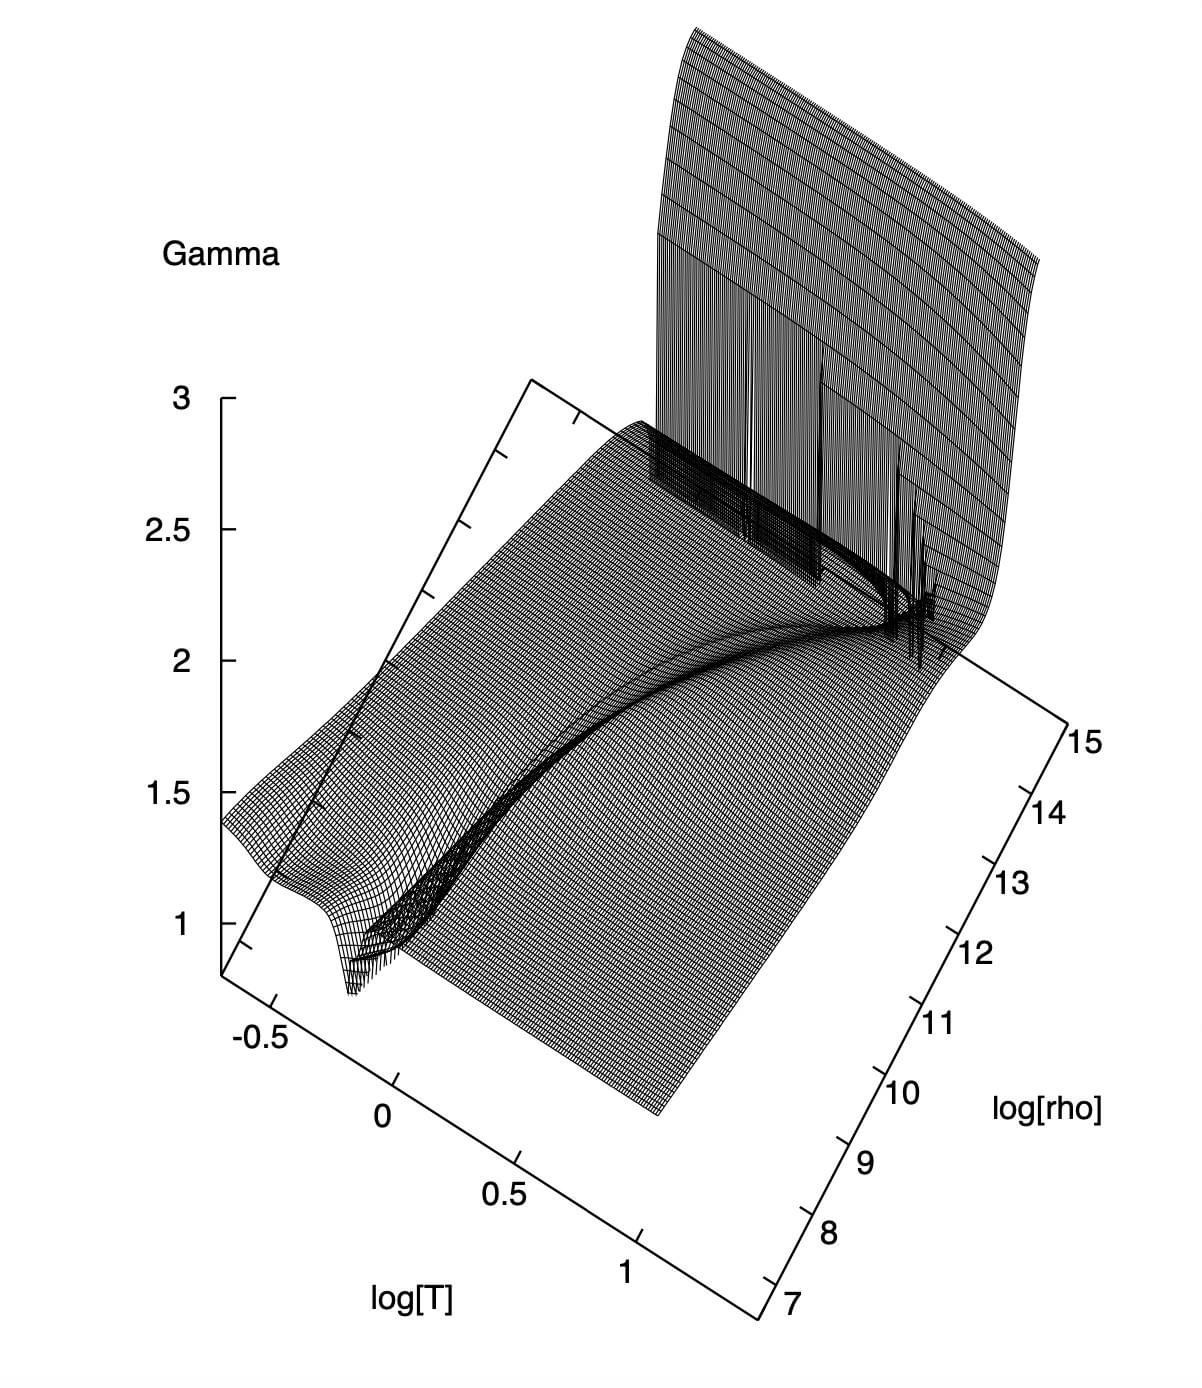
\includegraphics[width=\linewidth]{lattimer.png}
  \caption{A plot of the $\gamma_c$ value returned by the Lattimer-Swesty equation of state, as a function of density (g cm$^{-3}$) and temperature (MeV) for $Y_e = 0.5$. Note that the value of $\gamma_c$ differs significantly from that of an ideal  relativistically degenerate  ($\gamma_c = 4/3$) gas, as is often assumed in simplified treatments of the neutron star mass in introductory astrophysics classes. Also note the sharp increase in the ``stiffness'' of the equation of state as the density approaches nuclear density values  $\sim 10^{15}$ g cm$^{-3}$, responsible for the ``bounce'' that occurs in core collapse supernova simulations.  The softening of the equation of state along the ``ridge'' is due to the formation of nuclei.  (courtesy Todd Thompson, PhD thesis) }
  \label{fig:lattimer}
\end{marginfigure}


We mentioned that the Helmholtz and nuclear equations of state are  {\it real} equations of state. A consequence of such a real equation of state is that two distinct exponents, $\gamma_e$ and $\gamma_c$, must be identified, from the pressure relation $p = (\gamma_e - 1) \rho \epsilon_{\rm int}$ and the sound speed relation $c_s = \left ( \gamma_c p / \rho  \right)^{1/2}$, respectively. Only the second of these is a genuine adiabatic exponent: $\gamma_c = (\partial \ln p / \partial \ln \rho)_s$ is what Chandrasekhar calls $\Gamma_1$, whereas $\gamma_e$ is an {\it effective} exponent constructed from the total internal energy rather than from a derivative taken along an adiabat.\marginnote{A real equation of state in fact requires three exponents $\Gamma_1, \Gamma_2, \Gamma_3$ in general, all of which coincide with $\gamma$ for an ideal gas. See Chandrasekhar, ``An Introduction to the Study of Stellar Structure,'' \S II, or Cox \& Giuli, ``Principles of Stellar Structure,'' \S 9.} For an ideal equation of state, it is easy to show from Equation \ref{eqn:ideal_gas} that these two exponents are the same, $\gamma_c = \gamma_e = \gamma$. In a real equation of state, including both Helmholtz and other nuclear equations of state, the exponents will in general differ, and the numerical hydrodynamics solvers  employed will generally require both. As a consequence, the solvers must be carefully crafted to self-consistently utilize the appropriate exponents  in precisely the correct locations. When the coarser approximation of an ideal equation of state is made by researchers, frequently the underlying reason is the absence of such a self-consistent numerical hydrodynamics solver in the code being used.

\subsection{Characteristic Speeds, Hyperbolicity, and the Timestep}

We have twice now called the hydrodynamical equations {\it hyperbolic} without saying what this means or where it comes from. It is worth a page, because the answer is precisely what sets the timestep of every simulation you will ever run.

Take the one-dimensional Euler equations, written in the primitive variables $\vec{q} = (\rho, v, p)$ of \S 1.3 and with gravity switched off. Using the equation of state to eliminate the internal energy in favor of the pressure, they can be assembled into the quasi-linear form

\begin{equation}
\frac{\partial \vec{q}}{\partial t} + \mathsf{A}(\vec{q}) \frac{\partial \vec{q}}{\partial x} = 0, \qquad
\mathsf{A} = \begin{pmatrix}
v & \rho & 0 \\
0 & v & 1/\rho \\
0 & \rho c_s^2 & v
\end{pmatrix}
\end{equation}
%
where the {\it adiabatic sound speed} is

\begin{equation}
c_s = \left[ \left( \frac{\partial p}{\partial \rho} \right)_{\! s} \right]^{1/2} = \left( \frac{\gamma_c \, p}{\rho} \right)^{1/2}
\end{equation}
%
A system of this form is called {\it hyperbolic} if the matrix $\mathsf{A}$ has real eigenvalues and a complete set of eigenvectors, and {\it strictly} hyperbolic if the eigenvalues are moreover distinct. Here the characteristic polynomial factors immediately,

\begin{equation}
(v - \lambda)\left[ (v-\lambda)^2 - c_s^2 \right] = 0 \quad \Longrightarrow \quad \lambda = v - c_s, \quad v, \quad v + c_s
\end{equation}
%
Three real, distinct eigenvalues -- so the Euler equations are strictly hyperbolic wherever $c_s > 0$. These are the speeds at which information physically propagates: the two acoustic waves running upstream and downstream at the sound speed relative to the flow, and the contact discontinuity, along which entropy and composition are simply carried along with the fluid at speed $v$. \marginnote{Contrast this with the elliptic Poisson equation of \S 1.4, where there is no propagation speed at all -- the potential everywhere responds instantaneously to the density everywhere. This is exactly why the two equations demand entirely different classes of numerical algorithm, and why gravity is typically solved as a separate operator-split step rather than being folded into the hydrodynamics update.}

The practical consequence is the Courant-Friedrichs-Lewy (CFL) condition. An explicit scheme cannot allow information to travel further than one cell in one timestep, so

\begin{equation}
\Delta t \le C_{\rm CFL} \frac{\Delta x}{\max_i \left| \lambda_i \right|} = C_{\rm CFL} \frac{\Delta x}{|v| + c_s}, \qquad C_{\rm CFL} \lesssim 1
\end{equation}
%
It is worth putting numbers to this once. For a simulation of a white dwarf interior with $c_s \sim 3 \times 10^8$ cm s$^{-1}$ resolved at $\Delta x \sim 10$ km on a $512^3$ grid, $\Delta t \sim 3 \times 10^{-3}$ s. Covering even a single dynamical time of a few seconds therefore requires of order a thousand steps -- and that estimate, not any consideration of memory, is what actually determines whether a given calculation is affordable.

\subsection{The Complete System}

It is worth pausing to collect what we have. The ideal, self-gravitating hydrodynamical system is

\begin{equation}
\boxed{
\begin{aligned}
\frac{\partial \rho}{\partial t} + \del\cdot (\rho\vec{v}) & = 0 \\
\frac{\partial(\rho {v}_i)}{\partial t} + \sum_j \frac{\partial}{\partial x_j} \left( \rho v_i v_j + p \, \delta_{ij} \right) & = \rho g_i \\
\frac{\partial (\rho E)}{\partial t} + \sum_i \frac{\partial}{\partial x_i} \left[ (\rho E + p) v_i \right] & = \sum_i \rho g_i v_i \\
\del^2 \Phi = 4\pi G \rho, \qquad \vec{g} & = -\del\Phi \\
p & = p(\rho, \epsilon_{\rm int}, X_i)
\end{aligned}
}
\end{equation}

Counting is instructive. In $D$ dimensions the unknowns are $\rho$, the $D$ components of $\vec{v}$, $p$, $\rho E$, and $\Phi$ -- $D+4$ in all. The equations are continuity (one), momentum ($D$), energy (one), Poisson (one), and the equation of state (one) -- also $D+4$. \marginnote{The definition $\rho E = \rho\epsilon_{\rm int} + \frac{1}{2}\rho v^2$ is what ties $\epsilon_{\rm int}$ to the evolved variable $\rho E$, and is not an independent equation. This is exactly the ``conservative to primitive'' inversion performed at every timestep by every code.} The system is closed, and that is precisely the content of the statement that the equation of state {\it closes} the hydrodynamical equations. Supply initial conditions and boundary conditions, and the evolution is determined.

\subsection{A Remark on the Derivation of the Equations of Fluid Mechanics and the Connection to Hilbert's Sixth Problem}


In our approach to deriving the equations of fluid mechanics, we have adopted a macroscopic point of view of the system -- that is, we do not begin with the underlying atomic structure of matter, and instead simply assume the existence of a continuous fluid material.  There are other routes to the equations of fluid mechanics which begin with the underlying microscopic description of the atomistic structure of matter. One of the most rigorous begins with the more fundamental Boltzmann equation for distribution functions of a system of interacting particles in non-equilibrium statistical mechanics, and from this derives an infinite hierarchy of equations,  using the Chapman-Enskog procedure derived by Chapman and Enskog (and, in a distinct but closely related expansion, by Hilbert), or the BBGKY hierarchy, developed by Bogoliubov, Born, Green, Kirkwood, and Yvon. The Chapman-Enskog procedure assumes a perturbative expansion about a thermalized solution, which breaks down in some cases -- for example, near shock interfaces. The procedure nonetheless establishes key relations between viscous and diffusive coefficients, among others. The BBGKY hierarchy is a non-perturbative relation between $N$ particle distribution functions, but some additional assumptions are needed to close the otherwise infinite system of equations and yield the Navier-Stokes (or Euler) equations of fluid mechanics.

These approaches address one part of  Hilbert's famous sixth problem, which aimed to axiomatize all of physics.  As a first step in this bold program, Hilbert suggested obtaining ``mathematically the limiting processes [...] which lead from the atomistic view to the laws of motion of continua." Hilbert's sixth problem, even in the special case of the Navier-Stokes or Euler equations, is considered largely unsolved from a mathematically rigorous standpoint still today. \footnote {See this \href{https://www.quantamagazine.org/famous-fluid-equations-are-incomplete-20150721/} {Quanta Magazine article} for a well-written popular introduction to mathematical issues related to the fluid equation derivations, and \href {https://arxiv.org/abs/1803.03599} {A. Gorban, 2018} or \href {https://doi.org/10.1090/bull/1650 }{I. Gallagher, 2019}, for more technical discussions. The Gorban reference is the introduction to an entire volume dedicated to Hilbert's sixth problem.}  Surprises continue to be found, particularly in the low density regime when the particle mean free path length is not much smaller than the length scales of interest. It is unclear what impact if any these mathematical developments have upon actual astrophysical processes; in some applications, the fluid approximation breaks down, and one must resort to a plasma physics treatment utilizing the full Boltzmann equations. In all likelihood, any breakdown will occur in extremely tenuous plasmas, and so for our discussion of stellar astrophysics, we will simply assume the validity of the Euler equations.

\vfill\eject

%%%%%%%%%%%%%%%%%%%%%%
%%
%%  New section on MHD
%%
%%%%%%%%%%%%%%%%%%%%%%

\section{Magnetohydrodynamics}
Ideal MHD is an effective theory, reduced from full plasma physics. The simplest theory of {\it ideal MHD} makes several key assumptions:
\begin{enumerate}
    \item Fluid approximation \textemdash local thermodynamic quantities can be defined in the plasma, and important fluid variations are longer and slower with respect to microscopic plasma processes. For example, important fluid scales are much larger than the gyroradius and slower than the gyrofrequency. We also assume that all fluid quantities are spatially continuous, as we did for the fluid equations.

    \item In a plasma, Ohm's Law locally and instantaneously relates the electric field and current. Ideal MHD further assumes perfect conductivity.

    \item The plasma is completely ionized and is charge neutral.

    \item The flow is non-relativistic (terms of order $\frac{v^2}{c^2}$ and higher can be dropped).
\end{enumerate}
%
Each of these assumptions can be relaxed depending on the application at hand. For example, in regions around neutron stars or black holes, one can develop special relativistic (or even general relativistic) MHD which drops the last assumption entirely. One may also include finite resistivity and  partial ionization in dense regions of molecular gas in star forming regions, resulting in the two fluid or the Hall MHD approximations. In these notes, however, we will focus on the case of  ideal MHD of a single fluid, which hold to an excellent degree of approximation within stellar interiors as we discuss below.

Because a great deal of what follows consists of dropping terms, it is worth setting down at the outset exactly which quantities we are treating as small, and how small. Everything in this section follows from a single consistent ordering:

\begin{center}
\fbox{
\begin{minipage}{0.90\linewidth}
{\bf MHD assumptions.} With $L$ the characteristic length scale of gradients and $u \equiv \max\left(v, c_s, v_A\right)$ the fastest characteristic signal speed,
\begin{align*}
\text{(i)} \quad & \frac{u}{c} \ll 1 && \text{all signal speeds non-relativistic} \\
\text{(ii)} \quad & \sigma \rightarrow \infty && \text{perfect conductivity} \\
\text{(iii)} \quad & \rho_e \rightarrow 0 && \text{quasi-neutrality}
\end{align*}
and all quantities are retained consistently to first order in $u/c$.
\end{minipage}
}
\end{center}

Two further orderings are frequently listed alongside these as though they were independent assumptions: that the electric field is weak, $|\E|/|\B| \sim v/c$, and that the fields evolve on the dynamical time, $\partial / \partial t \sim u/L$. They are not independent. The first follows in \S 2.1 from perfect conductivity alone, and the second from it by way of Faraday's law in \S 2.4. We flag them here only so that the logic of the $u/c$ expansion is visible in advance. \marginnote{It is tempting to write the second of these as $\partial / \partial t \sim v/L$, on the grounds that the field is simply carried around by the fluid. That is correct for a purely advective flow, but it fails badly in a low-$\beta$ plasma, where the Alfv\'en speed can vastly exceed the fluid speed and the field instead evolves on $L/v_A$. What actually matters for discarding the displacement current is that the {\it fastest} signal speed be non-relativistic. This is why relativistic MHD is required in, say, a magnetar magnetosphere, where $v_A \rightarrow c$ even though the plasma itself is barely moving.}

\subsection{Ohm's Law and the Electric Field in Ideal MHD}

Consider the Lorentz transformation of $\E$ and  $\B$. Let's notate the center-of-mass frame in which the fluid is locally at rest as the primed frame, and the lab frame as the unprimed frame. The fluid -- and hence the primed frame -- moves with velocity $\vec{v}$ {\it as measured in the lab frame}.\marginnote{It is worth being pedantic about this, because every sign in what follows hinges on it. The primed frame moves at $+\vec{v}$ relative to the unprimed frame. Getting this backwards flips the sign of the induced electric field, and with it the sign of the entire induction equation.}

\begin{align}
\E_{\parallel}^{\prime} & = \E_{\parallel} \\
\B_{\parallel}^{\prime} & = \B_{\parallel} \\
\E_{\bot}^{\prime} & = \gamma \left( \E_\bot + \frac{\vec{v}}{c}
\times \B  \right) \\
\B_{\bot}^{\prime} & = \gamma \left( \B_\bot - \frac{\vec{v}}{c} \times \E  \right)
\end{align}

Here, the parallel and perpendicular components refer to the components parallel and perpendicular to the velocity, eg,  $\E_\parallel = (\E \cdot \hat{v})\hat {v}$, and $\E = \E_\parallel + \E_\bot$, where $\hat {v}$ is the unit vector in the direction of the velocity vector, $\hat {v} = \vec {v} / v$.  Then we can write the Lorentz transformation as a single vector transformation:
%An equivalent transformation uses $\E = \E_\parallel + \E_\bot$, $\E_\parallel = (\E \cdot \vec{v})$

\begin{align}
\E^\prime & = \gamma \left( \E + \frac{\vec{v}}{c}
\times \B  \right) - (\gamma - 1) \left(\E \cdot \hat {v}   \right) \hat{v} \\
\B^\prime & = \gamma \left( \B - \frac{\vec{v}}{c}
\times \E  \right) - (\gamma - 1) \left(\B \cdot \hat {v}   \right) \hat{v}
\end{align}
%
\marginnote{These are readily checked by decomposing into parallel and perpendicular pieces, and noting that $\vec{v} \times \B$ is purely perpendicular to $\vec{v}$, so that the subtracted term removes exactly the unwanted factor of $\gamma$ from the parallel component.}


But, these are the exact Lorentz transformations, while the non-relativistic fluid equations we derived in \S 1 are {\it only Galilean invariant}. If we are to build a consistent non-relativistic theory, we must therefore expand in $v/c$ and keep terms only to a fixed order throughout. Expanding $\gamma$,

\begin{align}
    \gamma & = \frac{1}{\sqrt{1-\frac{v^2}{c^2}}} \simeq 1 + \frac{1}{2} ~ \frac{v^2}{c^2} = 1 + \mathcal{O}\left(\frac{v^2}{c^2}\right)
\end{align}

Working to first order in $v/c$, and neglecting terms $\mathcal{O}\left(v^2/c^2\right)$,

\begin{align}
    \E^\prime & = \E + \frac{\vec{v}}{c} \times \B  \label{eqn:Eprime} \\
    \B^\prime & = \B - \frac{\vec{v}}{c} \times \E \; = \; \B + \mathcal{O}\left(\frac{v^2}{c^2}\right) \B \; \simeq \; \B \label{eqn:Bprime}
\end{align}
%
The second line requires a word of care. The correction $\frac{\vec{v}}{c} \times \E$ is only {\it first} order in $v/c$, and so does not vanish merely because the flow is slow -- it is negligible because $|\E| \sim (v/c)|\B|$, the weak-field ordering flagged above, which demotes it to second order. We are about to establish exactly that, and note that we establish it {\it without} appealing to Equation \ref{eqn:Bprime}, so the argument is not circular.

In a perfectly conducting charge-neutral medium, $\abs{\E^\prime}=0$ in the center-of-mass frame, since charges can freely move to cancel out the electric field.  To see this slightly more formally, write Ohm's law in terms of the electric current $\vec {j}_e^\prime$ in the center-of-mass frame as $\vec {j}^\prime_e = \sigma \vec {E}^\prime$. Then, inverting Equation \ref{eqn:Eprime},

\begin{align}
\E & = \E^\prime - \frac{\vec{v} }{c}\times \B = \frac{\vec{j}_e^\prime}{\sigma} - \frac{\vec{v}}{c}\times \B
\end{align}

As we will learn later in \S \ref {sec:alfven},  for a perfectly conducting fluid, the magnetic field remains frozen into the fluid. For finite conductivity $\sigma$, the magnetic field will not remain frozen into the fluid, but will instead diffuse outwards. We can therefore ask ourselves what might happen in a perfect conductor. Just as with any diffusion process, the timescale $\tau$ scales quadratically with the length scale $L$: $\tau = 4 \pi \sigma L^2 / c^2$.\footnote {See J.D. Jackson Electrodynamics, 2nd edition, \S 10.3.} The question of whether non-ideal conductivity is needed or not therefore amounts to a question of whether we are interested in timescales comparable to $\tau$ or not. %A 1 cm sphere of copper has $\tau \sim 1$ s, but f
For the center of a white dwarf with $\sigma \sim 10^{22}$ s$^{-1}$ and a length scale set by its radius, $L = 5 \times 10^3$ km, the timescale to diffuse the field through to the surface exceeds the Hubble time, $\tau \sim 10^{12}$ yr.\footnote {See \url{https://arxiv.org/abs/astro-ph/9604165} for a calculation of the conductivity.} Even if we were to consider a small chunk of the interior with $L = 1 $ km, $\tau \sim 5 \times 10^4$ yr. Generally speaking, the diffusion timescale for stellar interiors is tremendously longer than the timescales we would be interested in simulating over a dynamical timescale, and the ideal conductor assumption is well-justified. In some phases of the interstellar medium, such as  the partially-ionized molecular gas within giant molecular clouds, non-ideal MHD effects are important even over a dynamical timescale of the cloud.

 For a perfect conductor, $\sigma\to \infty$, and the Ohmic term on the right can be dropped.
\begin{align}
    \E & = - \frac{\vec{v}}{c} \times \B
\label{eqn:ideal_ohm}
\end{align}
%
This is the {\it ideal Ohm's law}: in ideal MHD the electric field is not an independent dynamical field at all, but is entirely determined by the fluid velocity and the magnetic field. Note that it was obtained from perfect conductivity and the $O(v/c)$ transformation of $\E$ alone -- so it {\it establishes} the ordering $|\E|/|\B| \sim v/c$ rather than assuming it, and retroactively justifies the step taken in Equation \ref{eqn:Bprime}.

\subsection{The Displacement Current}

Equation \ref{eqn:ideal_ohm} implies an electric field  $\abs{\E}\simeq \frac{v}{c}\ \abs {\vec {B}}$ in the lab frame. Now consider Ampere's Law:

\begin{equation}
\del \times \B = \frac{4\pi }{c}~\vec{j}_e + \frac{1}{c}~\frac{\partial\E}{\partial t}
\end{equation}
where $\vec {E}$ and $\vec {B}$ represent the electric and magnetic fields, respectively, $\vec{j}_e$ is the electric current density, and $\frac{1}{c}~\frac{\partial\vec{E}}{\partial t}$ is the displacement term.\footnote {Note that we utilize Gaussian electromagnetic units -- see appendix for a comparison of Gaussian and SI electromagnetic units.}
%
We can estimate the relative magnitude of the displacement term in terms of a characteristic timescale $\tau$ of the variation of the fields:

\begin{align}
\frac{1}{c}~\abs{\frac{\partial \E}{\partial t}} & \simeq \frac{1}{c}~\frac{E}{\tau} \simeq \frac{1}{c}~\frac{v}{c}~\frac{B}{\tau}
\end{align}

Let's compare this term with $\del \times \B$, writing the characteristic lengthscale of gradients as $L$ and the characteristic dynamical timescale $\tau \sim L / v$,\marginnote{Here we take the flow to be advective, so that $u = v$. For a magnetically dominated plasma one should instead use $\tau \sim L/v_A$, and repeating the estimate gives a ratio $v_A^2/c^2$ in place of $v^2/c^2$. The displacement current is negligible precisely when the fastest signal speed is non-relativistic, which is assumption (i).}
\begin{align}
\frac{\displaystyle\frac{1}{c} \abs{\frac{\partial \E}{\partial t}} }{\abs{\del \times \B}} & \simeq \frac{\displaystyle\frac{1}{c}~\frac{v}{c}~\frac{B}{\tau}}{\displaystyle\frac{B}{L}} \simeq \frac{v}{c^2}~\frac{L}{\tau} \simeq \frac{v^2}{c^2}
\end{align}
%

So the displacement term can be neglected, and one obtains
\begin{align}
    \del \times \B & = \frac{4\pi}{c}\vec{j}_e
\end{align}

Or, in other words, non-relativistic ideal MHD current densities are always obtainable directly from the magnetic field:
\begin{align}
    \vec{j}_e &= \frac{c}{4\pi}~\del \times \B
\label{eqn:current}
\end{align}
%
In ideal MHD, the magnetic field takes center stage. Both the electric field and the current density take a less direct role than in the full Maxwell theory, though current densities are often a nice way to visualize the dynamics of the magnetic field.

Furthermore,
\begin{align}
    \del \cdot \vec{j}_e & = \frac{c}{4\pi}~\del \cdot \left(\del \times \B \right) = 0
\end{align}

Non-relativistic MHD currents always close upon themselves, and have no local sources or sinks. This is entirely consistent with the assumed charge neutrality: charge conservation reads $\partial \rho_e / \partial t + \del\cdot\vec{j}_e = 0$, and a divergence-free current is exactly what is required to keep $\rho_e$ pinned at zero.
% in 2D, and closing of currents not an issue in 3D.

\subsection{Charge Neutrality and the Drift Current}

The drift velocities are also typically negligible between ions and electrons. Let's write the electric charge density as $\rho_e$, so as not to confuse it with the mass density $\rho$:

\begin{equation}
\rho_e = \bar {Z} e n_i - en_e = 0 \quad \text{by charge neutrality}
\end{equation}
%
Here $\bar {Z}$ is the ionic mean (weighted by number) charge. It follows that $n_i = n_e / \bar {Z}$ in any charge-neutral medium.

Now we reach a somewhat subtle but tremendously important point about the physical origin of the fields in the ideal MHD approximation. Namely, {\it even though the fluid is assumed to be charge neutral, an ionized fluid can still possess an electric current due to the drift current between the ions and electrons}. If the mean velocity of the electrons $\vec{v}_e$ differs from the ions $\vec{v}_i$, the net electric current density $\vec {j}_e$ is
\begin{align}
\vec{j_e} & = \bar {Z}en_i \vec{v}_i - en_e \vec{v}_e \\
& = en_e \vec{v}_i - en_e\vec{v}_e = -en_e (\vec{v}_e - \vec{v}_i) = -en_e \vec{v}_e^\prime
\end{align}
%
Here $\vec{v}_e^\prime =  (\vec{v}_e - \vec{v}_i)$ is the {\it drift velocity} of the electrons with respect to the ions -- that is, the electron velocity measured in the frame comoving with the ions, which is why it carries the subscript $e$ and the prime. The minus sign is simply the negative charge of the electron: current flows opposite to the direction the electrons drift.

Let's estimate the drift velocity $\vec{v}_e^\prime$ that arises near the surface of a high field magnetized white dwarf (HFMWD), a class of highly magnetized white dwarfs that are thought to originate at least in part from white dwarf mergers. Let's take the white dwarf to be 1 $M_{\odot}$, $R = 5800$ km, with a  DA (hydrogen-dominated) envelope,  surface field $B \sim 10^9$ G, $\rho \sim 1$ g cm$^{-3}$, $n_e \sim 6 \times 10^{23}$ cm$^{-3}$, scale height $h \sim k T /  (m g) \sim 200$ m:

\begin{align}
\vec{j}_e & = \frac{c}{4\pi} ~\del \times \B  \\
\abs{\vec{j}_e} & \simeq e n_e {v}_e^\prime \\
\frac{c}{4\pi}~\abs{\del \times \B} & \simeq \frac{c}{4\pi}~\frac{B}{h} \\
v_e^\prime &\simeq \frac{c}{4\pi e n_e}~\frac{B}{h} \simeq 1 ~\text{cm/s}
\end{align}
%
\marginnote{These numbers describe the ionized envelope a little below the photosphere; note that $h \sim 200$ m corresponds to $T \sim 10^5$ K at $\log g = 8$. At the photosphere proper one has instead $\rho \sim 10^{-2}$ g cm$^{-3}$ and $h \sim 25$ m, and the same estimate gives $v_e^\prime \sim 2$ m/s. Either way the conclusion is unchanged, which is the useful thing about an estimate this lopsided.}

Consequently, even a very strong gigagauss white dwarf magnetic field requires only a tiny drift velocity, far smaller than the fluid velocity or the sound speeds ($c_s \sim 30$ km/s) we are typically interested in simulating during dynamical processes.  Repeating the same estimate for a more typical stellar magnetic field, such as that observed in the solar photosphere, where $n_e \sim 6 \times 10^{13}~$cm$^{-3}$, $h\sim 1.5\times 10^{7}~$cm, and $B\sim 10^3~$G, one finds a drift velocity of only $\sim 5~\text{cm/s}$ -- five orders of magnitude below the photospheric sound speed of $\sim 8$ km/s.\marginnote{It is worth pausing on the fact that the solar photosphere, with a field a million times {\it weaker}, nonetheless demands a drift a little {\it larger} than the gigagauss white dwarf. The scaling is $v_e^\prime \propto B / (n_e h)$. The white dwarf's field is $10^6$ times stronger and its scale height $10^3$ times smaller, so it requires a current density some $10^9$ times larger -- but it has $10^{10}$ times as many electrons on hand to carry it, and the density wins. The lesson is that the drift velocity is set far more by how much charge is available than by how strong the field is. This is also why the photosphere is the less comfortable case of the two: it is only weakly ionized, with $\rho \sim 3\times10^{-7}$ g cm$^{-3}$ giving $n_{\rm tot} \sim 10^{17}$ cm$^{-3}$ but an ionization fraction of only $\sim 5\times10^{-4}$, most of those electrons donated by ionized metals rather than by hydrogen.} When modeling stellar interiors, we therefore usually adopt the \textit{single fluid approximation} for MHD, and assume electrons and ions  are comoving with the same velocity, with effectively zero drift velocity, $v_e^\prime=0$. All fluid velocities will be written simply as $\vec {v}$.\footnote{This assumption needs to be relaxed in the low-ionization gas in protostellar disks and the interstellar medium.}

\subsection{Induction Equation and the Solenoidal Constraint}

From Faraday's Law,

\begin{align}
    \del \times \E & = - \frac{1}{c}~\frac{\partial \B}{\partial t} \\
    \del \times \left( - \frac{\vec{v}}{c} \times \B  \right) & = - \frac{1}{c}~\frac{\partial \B}{\partial t}
%  \frac{\partial \B}{\partial t} & = \del \times (\vec{v} \times \B )
\end{align}

%In the single fluid approximation, ions and electrons are assumed to be comoving, so we can also write $\vec{v}_i=\vec{v}$, the single fluid velocity,
where we have substituted the ideal Ohm's law, Equation \ref{eqn:ideal_ohm}. Note that Faraday's law is used here in its exact form -- no appeal to the displacement-current estimate of \S 2.2 is required -- so what follows rests only on ideal Ohm's law. This yields the magnetic induction equation governing the time evolution of the magnetic field in the ideal MHD approximation.

\begin{equation}
  \boxed{  \frac{\partial \B}{\partial t} = \del \times (\vec{v}\times \B ) }
\label{eqn:induction}
\end{equation}
%
This is also where the second of the two orderings noted at the start of \S 2 is earned. Scaling the right-hand side gives $|\partial \B / \partial t| \sim v B / L$, so the field evolves on the advective time $L/v$ -- or, once the momentum equation is coupled in and the plasma is free to support Alfv\'en and magnetosonic waves, on $L/u$ with $u$ the fastest of the characteristic speeds. It is not an independent assumption about how quickly the fields are permitted to vary.

Had we not taken $\sigma \to \infty$, the Ohmic term $\vec{j}_e^\prime/\sigma$ would have survived, and using Equation \ref{eqn:current} to eliminate the current would have given instead the {\it resistive} induction equation

\begin{equation}
\frac{\partial \B}{\partial t} = \del \times (\vec{v}\times \B ) + \eta \, \del^2 \B , \qquad \eta \equiv \frac{c^2}{4\pi\sigma}
\label{eqn:resistive_induction}
\end{equation}
%
where $\eta$ is the magnetic diffusivity. The diffusion timescale quoted above is now simply $\tau = L^2/\eta = 4\pi\sigma L^2/c^2$, as it must be for any diffusion equation, and the dimensionless ratio of the two terms on the right defines the {\it magnetic Reynolds number}

\begin{equation}
Re_M \equiv \frac{vL}{\eta}
\end{equation}
%
Ideal MHD is the statement $Re_M \rightarrow \infty$. In stellar interiors $Re_M$ is routinely of order $10^{10}$ or larger, which is what makes the approximation so good.

The induction equation must be accompanied by the solenoidal constraint,

\begin{equation}
\boxed{ \del\cdot\B = 0 }
\label{eqn:divb}
\end{equation}
%
This is not an additional dynamical equation but a {\it constraint} on the initial data, and the induction equation is precisely what preserves it. Taking the divergence of Equation \ref{eqn:induction},

\begin{equation}
\frac{\partial}{\partial t}\left( \del\cdot\B \right) = \del\cdot\left[ \del\times(\vec{v}\times\B) \right] = 0
\end{equation}
%
so that if $\del\cdot\B = 0$ initially, it remains zero for all time. \marginnote{This innocent-looking statement is the source of an enormous amount of effort in numerical MHD. A discretized curl does {\it not} in general have an exactly vanishing discretized divergence, so $\del\cdot\B$ accumulates numerical error, and a nonzero $\del\cdot\B$ produces an unphysical force parallel to $\B$ that can wreck a simulation. The two standard cures are {\it constrained transport}, which stores the field on cell faces in a staggered arrangement for which the discrete divergence vanishes identically to machine precision, and {\it divergence cleaning}, which advects and damps the error away. Every production MHD code implements one or the other.}

\subsection{The MHD Momentum and Energy Equations}

So far the magnetic field has been a passenger: Equation \ref{eqn:induction} tells us how $\B$ responds to $\vec{v}$, but not yet how $\vec{v}$ responds to $\B$. The missing ingredient is the Lorentz force per unit volume acting on the fluid, $\frac{1}{c}\vec{j}_e \times \B$, which by Equation \ref{eqn:current} is expressible entirely in terms of the magnetic field. Using the vector identity $\del\left(\frac{1}{2}B^2\right) = (\B\cdot\del)\B + \B\times(\del\times\B)$,

\begin{equation}
\frac{1}{c}\vec{j}_e \times \B = \frac{1}{4\pi}\left(\del\times\B\right)\times\B = \underbrace{-\del\left(\frac{B^2}{8\pi}\right)}_{\text{magnetic pressure}} + \underbrace{\frac{1}{4\pi}\left(\B\cdot\del\right)\B}_{\text{magnetic tension}}
\label{eqn:lorentz}
\end{equation}
%
This decomposition is, in my view, the single most useful piece of intuition in all of MHD. The first term says that a magnetic field pushes sideways on the fluid exactly as an isotropic pressure $B^2/8\pi$ would; the second says that field lines behave like elastic strings under tension $B^2/4\pi$, and pull back when bent. \marginnote{The magnetic tension term is what supplies the restoring force for the Alfv\'en waves described in \S \ref{sec:alfven}, and the magnetic pressure term is what allows a magnetized region to support itself against gravity even at low gas pressure. The ratio of the two pressures defines the {\it plasma beta}, $\beta \equiv 8\pi p / B^2$, which is the standard measure of whether a plasma is dominated by its gas or its field.}

Adding Equation \ref{eqn:lorentz} to the right-hand side of the momentum equation and using $\del\cdot\B = 0$ to fold both terms back inside a divergence, we obtain the ideal MHD momentum equation in conservative form:

\begin{equation}
\boxed{ \frac{\partial(\rho v_i)}{\partial t} + \sum_j \frac{\partial}{\partial x_j}\left[ \rho v_i v_j + \left( p + \frac{B^2}{8\pi} \right)\delta_{ij} - \frac{B_i B_j}{4\pi} \right] = \rho g_i }
\label{eqn:mhd_momentum}
\end{equation}
%
The bracketed quantity is the total momentum flux density tensor; the magnetic part of it, $\frac{1}{4\pi}\left( \frac{1}{2}B^2 \delta_{ij} - B_i B_j \right)$, is the Maxwell stress tensor. Note that unlike the ideal gas pressure, it is emphatically {\it not} isotropic -- the field picks out a direction, and the fluid knows it.

The energy equation acquires the magnetic energy density $B^2/8\pi$ and the Poynting flux $\frac{c}{4\pi}\E\times\B$, which upon substituting the ideal Ohm's law becomes $\frac{B^2}{4\pi}\vec{v} - \frac{(\vec{v}\cdot\B)\B}{4\pi}$. Writing the total energy density as $\rho E_{\rm tot} = \rho\epsilon_{\rm int} + \frac{1}{2}\rho v^2 + \frac{B^2}{8\pi}$,

\begin{equation}
\boxed{ \frac{\partial (\rho E_{\rm tot})}{\partial t} + \del\cdot\left[ \left( \rho E_{\rm tot} + p + \frac{B^2}{8\pi} \right)\vec{v} - \frac{(\vec{v}\cdot\B)\B}{4\pi} \right] = \rho \, \vec{g}\cdot\vec{v} }
\label{eqn:mhd_energy}
\end{equation}
%
Equations \ref{eqn:continuity}, \ref{eqn:mhd_momentum}, \ref{eqn:mhd_energy}, \ref{eqn:induction}, and \ref{eqn:divb}, together with the equation of state, constitute the complete system of ideal MHD.

Finally, the characteristic analysis of \S 1.6 generalizes, though the algebra is considerably less pleasant. Introducing the {\it Alfv\'en speed}

\begin{equation}
v_A \equiv \frac{B}{\sqrt{4\pi\rho}}
\end{equation}
%
the one-dimensional ideal MHD system is hyperbolic with seven characteristic speeds rather than three: the entropy mode travelling at $v$, a pair of Alfv\'en waves at $v \pm v_{A,x}$, and two pairs of magnetosonic waves at $v \pm c_{f}$ and $v \pm c_{s\ell}$, where the fast and slow speeds satisfy
\begin{equation}
c_{f,s\ell}^2 = \frac{1}{2}\left[ \left( c_s^2 + v_A^2 \right) \pm \sqrt{\left( c_s^2 + v_A^2\right)^2 - 4 c_s^2 v_{A,x}^2} \right]
\end{equation}
%
The CFL condition is then set by the fast magnetosonic speed, $\Delta t \le C_{\rm CFL}\Delta x / (|v| + c_f)$. \marginnote{Note that the MHD system is {\it not} strictly hyperbolic: the slow and Alfv\'en speeds coincide when $\B$ is perpendicular to the direction of propagation, and the fast and Alfv\'en speeds coincide when it is parallel. These degeneracies are harmless physically but are a genuine nuisance for Riemann solvers, and much of the intricacy of modern MHD schemes exists to handle them gracefully.}

\subsection{Alfv\'en Theorem}
\label{sec:alfven}
The Alfv\'en Theorem states that in the ideal MHD approximation, the magnetic flux is ``frozen'' into comoving fluid elements. Writing a surface comoving with the fluid as $S(t)$, the magnetic flux threading it is $\Phi (S)$,

\begin{align}
    \Phi (S) & = \int_{S(t)} \B \cdot \mathrm{d}\vec{S} \\
    \frac{\mathrm{d}\Phi (S)}{\mathrm{d}t} & = 0
\end{align}

\begin{marginfigure}
  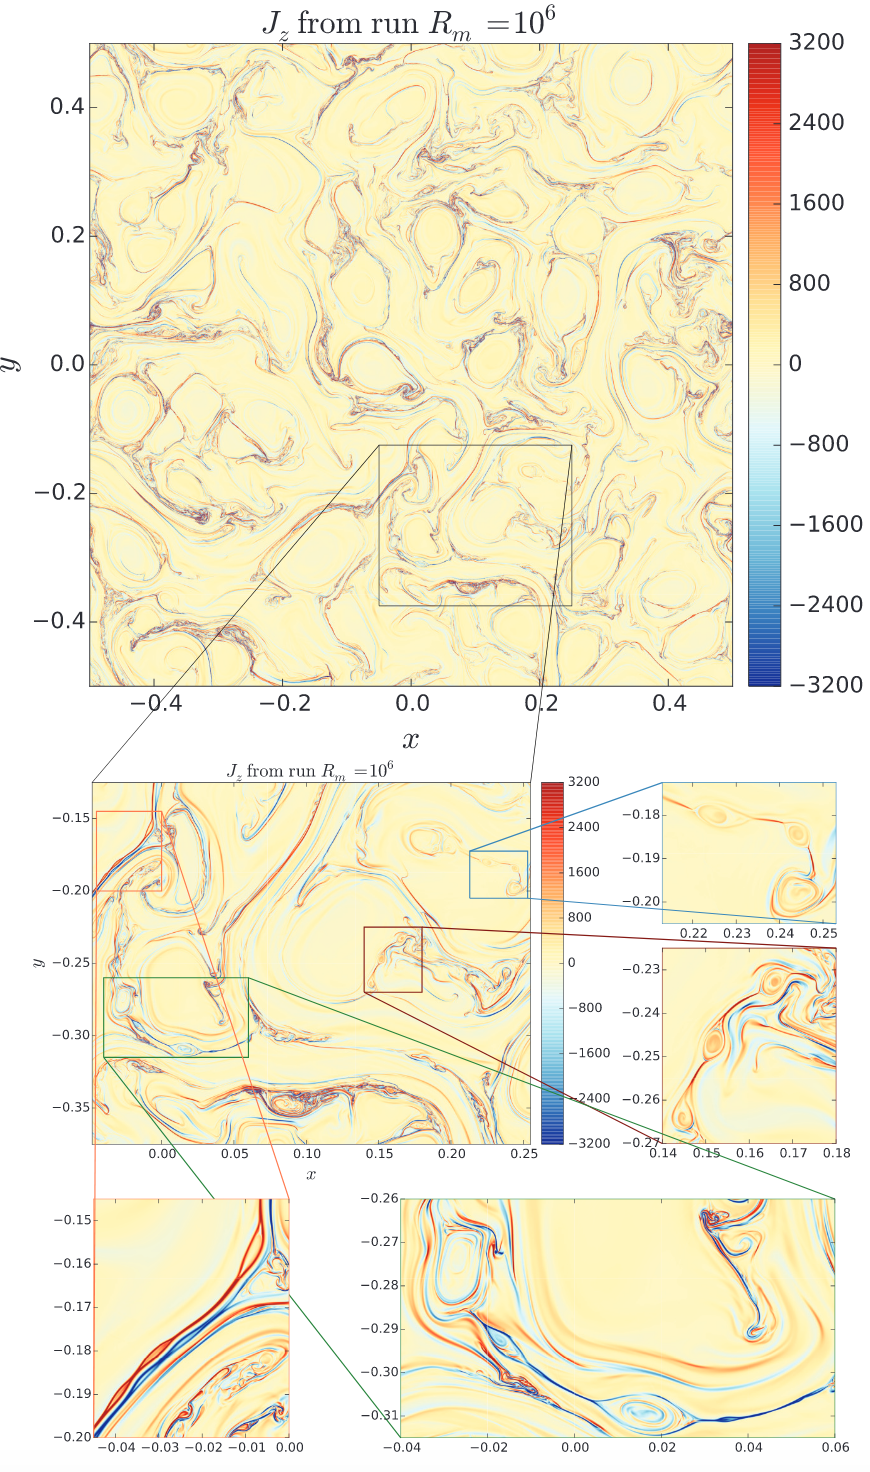
\includegraphics[width=\linewidth]{current_sheets_dong18.png}
  \caption{Current density from a high magnetic Reynolds number 2D MHD simulation at Lundquist number $S = 10^6$, showing reconnection and the formation of plasmoids \url {https://doi.org/10.1103/PhysRevLett.121.165101}.}
  \label{fig:plasmoids}
\end{marginfigure}

The proof takes three lines and is worth seeing, because it makes clear exactly where the induction equation enters. The flux through a comoving surface changes for two reasons: the field itself may change in time, and the boundary of the surface sweeps through space, so that the surface encloses different field lines at different times. In a time $\mathrm{d}t$, an element $\mathrm{d}\vec{\ell}$ of the boundary sweeps out a ribbon of area $(\vec{v}\,\mathrm{d}t) \times \mathrm{d}\vec{\ell}$, and so

\begin{align}
\frac{\mathrm{d}\Phi}{\mathrm{d}t} & = \int_S \frac{\partial \B}{\partial t}\cdot\mathrm{d}\vec{S} + \oint_{\partial S} \B\cdot\left( \vec{v}\times\mathrm{d}\vec{\ell} \right) \\
& = \int_S \frac{\partial \B}{\partial t}\cdot\mathrm{d}\vec{S} - \oint_{\partial S} \left( \vec{v}\times\B \right)\cdot\mathrm{d}\vec{\ell} \\
& = \int_S \left[ \frac{\partial \B}{\partial t} - \del\times\left( \vec{v}\times\B \right) \right]\cdot\mathrm{d}\vec{S} \; = \; 0
\end{align}
%
where the second line uses the cyclic property of the scalar triple product, the third uses Stokes' theorem, and the final equality is precisely the induction equation, Equation \ref{eqn:induction}. \marginnote{Run the argument backwards and it is equally instructive: flux freezing is not an additional physical assumption layered on top of ideal MHD, but is {\it exactly equivalent} to it. Restoring the resistive term of Equation \ref{eqn:resistive_induction} leaves $\mathrm{d}\Phi/\mathrm{d}t = \eta\int_S \del^2\B\cdot\mathrm{d}\vec{S} \ne 0$, and the field slips through the fluid.}

The Alfv\'en Theorem has profound implications. Because the magnetic flux remains frozen to the fluid in the ideal MHD approximation, we can understand a myriad of complex physical effects simply and intuitively. As just one example, displacing the magnetic field perpendicular to its length generates a restoring force from the magnetic tension term of Equation \ref{eqn:lorentz}, and gives rise to incompressible MHD waves called Alfv\'en waves, propagating along the field at the Alfv\'en speed $v_A$.
The Alfv\'en Theorem also implies that the magnetic field topology is unchanged in ideal MHD, and points to some inherent limitations of this set of approximations. Turbulent dynamos, for instance, require that the magnetic field cascading down to small length scales eventually undergoes magnetic reconnection, which changes the topology of the field. At sufficiently high magnetic Reynolds number, turbulently folded magnetic sheets become extremely thin, and get chopped up, or reconnected,  into isolated islands of magnetic flux called ``plasmoids'' (Fig. \ref{fig:plasmoids}).
Reconnection is only possible in a resistive medium, which is formally beyond the ideal MHD approximation. However, numerical solutions of the ideal MHD equations also necessarily carry with them some finite {\it numerical} resistivity resulting from the discretization of the equations. This numerical resistivity can produce numerical reconnection, which mimics the effects of a physical resistivity -- though at an effective $Re_M$ set by the grid rather than by the plasma, which is a caveat always worth keeping in mind when interpreting such a simulation.

\section{Further Reading}

For the fluid equations themselves and their physical content, Landau \& Lifshitz, ``Fluid Mechanics,'' remains unmatched for compactness. For the numerical treatment of conservation laws, LeVeque, ``Numerical Methods for Conservation Laws,'' and Toro, ``Riemann Solvers and Numerical Methods for Fluid Dynamics,'' are the standard references; the latter is the more practical of the two if you intend to write a solver. For MHD, Goedbloed \& Poedts, ``Principles of Magnetohydrodynamics,'' gives a thorough treatment from the plasma physics side, while Shu, ``The Physics of Astrophysics, Vol. II: Gas Dynamics,'' is closest in spirit to these notes. For stellar equations of state, Cox \& Giuli, ``Principles of Stellar Structure,'' is still the most complete single source.

\vfill\eject




\appendix

\section  {A Note on SI and Gaussian  Units in Electromagnetism}

\subsection {SI Units}

When considering electromagnetism units, it is important to note that differing systems of units not only modify the physical units, but also the form of the equations themselves. In particular, there are multiple choices for electromagnetic units,  which are  manifest in  differences in the actual written form of Maxwell's equations. Consider Gauss's law, first in SI units, which has base dimensions of mass, length, time, and electric current (sometimes also called meters, kilograms, seconds, and Amperes units, or MKSA units).  The electric field due to a point charge is


\begin{equation}
\vec{E}_{\text{SI}} = \frac{1}{4\pi \epsilon_0} \frac{q_{\text{SI} } } {r^2}   \hat{r}
\end{equation}

In SI, the unit of the charge is the Coulomb, [q$_{\text{SI} }$]=\text{C}.\footnote {The [] notation used here is an operator that returns the units of the expression contained within.} Heaviside referred to this system as ``rationalized'' units, since the $4\pi$ factor coming from spherical geometry is subsumed into the coupling constant in Coulomb's law. Consequently, the electric flux through a closed surface is
\begin{equation}
\int \del \cdot \vec{E}_{\text{SI}}~\mathrm{d}V = \frac{1}{\epsilon_0} \int \rho_{e\text{,SI}}~\mathrm{d}V
\end{equation}
\begin{equation}
\oint \vec{E}_{\text{SI}}\cdot \mathrm{d}\vec{A} = \frac{1}{\cancel{4\pi}\epsilon_0}~\frac{q_{\text{SI}}}{\cancel{r^2}}~ 4\pi \cancel{r^2}  = \frac{q_{\text{SI}}}{\epsilon_0}
\end{equation}

%\[
%\frac{1}{\cancel{4\pi}\epsilon_0}~\frac{q}{\cancel{r^2}}~ 4\pi \cancel{r^2} = \frac{q}{\epsilon_0}
%\]

As a result, Gauss's law in SI units has no factors of $4 \pi$. The elimination of the geometric factors from Maxwell's equations in the older Gaussian unit system was in fact Heaviside's motivation in choosing rationalized units.

%\textbf{Divergence of the electric field:}
\begin{equation}
\del \cdot \vec{E}_{\text{SI}} = \frac{\rho_{e\text{,SI}}}{\epsilon_0}
\end{equation}

\subsection {Gaussian Electromagnetic Units}

In contrast, in Gaussian units, the base dimensions are chosen to be mass, length, and time.\footnote {The name ``Gaussian'' in fact goes all the way back to Gauss himself, who among numerous other achievements devised the first consistent system of electromagnetic units while undertaking geomagnetic measurements.} Electric charge and electric current are constructed from these base dimensions.  The electric field due to a point charge is written:

\begin{equation}
\vec{E}_{\text{Gauss}}  = \frac{q_{\text{Gauss}} }{r^2} \hat{r}
\end{equation}

In Gaussian units, the unit of charge is the statcoulomb or franklin (named in honor of Benjamin Franklin), [q$_{\text{Gauss}}$] = statC or Fr $\simeq 3.3\times 10^{-10}~\text{C}$. Note that in Gaussian units, there is no factor of $4\pi$ in Coulomb's law. This is analogous to how we treat Newtonian gravity, so Sommerfeld called this system ``conventional.''

\begin{equation}
\int \del \cdot \vec{E}_{\text{Gauss}}~\mathrm{d}V = 4\pi q_{\text{Gauss}}
\end{equation}
\begin{equation}
\oint \vec{E}_{\text{Gauss}} \cdot \mathrm{d}\vec{A} =  \frac{q_{\text{Gauss}}}{\cancel{r^2}}~4\pi\cancel{r^2} = 4\pi q_{\text{Gauss}}
\end{equation}

%\[
%\frac{q}{\cancel{r^2}}~4\pi\cancel{r^2} = 4\pi q_{\text{Gauss}}
%\]

The $4\pi$ geometric factor must instead be incorporated into Gauss's law:

\begin{equation}
\del \cdot \vec{E}_{\text{Gauss}} = 4\pi \rho_{e, \text{Gauss}}
\end{equation}

The appearance of the additional geometric factor in the more fundamental Maxwell equation is precisely what annoyed Heaviside and motivated him to develop rationalized units.



%\begin{table}[H]
%    \centering
%    \renewcommand{\arraystretch}{2}
%    \begin{tabular*}{\textwidth}{C{0.45\textwidth} | C{0.45\textwidth}}
%         \textbf{``Rationalized'' SI} & \textbf{``Conventional CGS''}

%    \end{tabular*}
%\end{table}

%         $\vec{E} = \frac{1}{4\pi \epsilon_0} \frac{q}{r^2} \hat{r}$ & $\vec{E} =  \frac{q}{r^2} \hat{r}$ \\


%         $[q]=$Coulomb & $[q] = $ statC or Fr $\simeq 3.3\times 10^{-10}~$C \\

%        \multicolumn{1}{p{0.45\textwidth}|}{
%        In rationalized units, the $4\pi$ factor coming from spherical geometry is subsumed into Coulomb's Law. Then,
%       } &
%        \multicolumn{1}{p{0.45\textwidth}}{
%        In conventional units, there is no factor of $4\pi$ in Coulomb's Law. This is analogous to how we treat Newtonian gravity, so Sommerfeld called this system ``conventional.'' The $4\pi$ geometric factor must instead be incorporated into Gauss's law:
%        }  \\


 %       $\int \vec{\nabla} \cdot \vec{E}~\mathrm{d}V = \frac{1}{\epsilon_0} \int \rho~\mathrm{d}V$ &
 %       $\int \vec{\nabla} \cdot \vec{E}~\mathrm{d}V = 4\pi q$ \\

 %       $\int \vec{E}\cdot \mathrm{d}\vec{A}$ = $\frac{q}{\epsilon_0}$ &
  %      $\int \vec{E}\cdot \mathrm{d}\vec{A} = 4\pi q$ \\

 %       $\frac{1}{\cancel{4\pi}\epsilon_0}~\frac{q}{\cancel{r^2}}~ 4\pi \cancel{}{r^2} = \frac{q}{\epsilon_0} $ &
  %      $\frac{q}{\cancel{r^2}}~4\pi\cancel{r^2} = 4\pi q$ \\

%        $\vec{\nabla} \cdot \vec{E} = \frac{q}{\epsilon_0} $ & $\vec{\nabla} \cdot \vec{E} = 4\pi q$

 %   \end{tabular*}
%\end{table}


The same situation extends to the other source terms in Maxwell's equations, the current density in Ampere's Law and the magnetic flux term in Faraday's Law:

\begin{table}
    \centering
    \renewcommand{\arraystretch}{2}
    \begin{tabular*}{0.9\textwidth}{ l @{\extracolsep{\fill}}  @{\extracolsep{\fill}}l }
        \underline {\textbf{SI} }& \underline {\textbf{Gaussian} }\\

    $\vec{\nabla}\times \vec{E}_{\text{SI}} = - \frac{\partial\vec{B}_{\text{SI}} }{\partial t}$ & $\vec{\nabla}\times \vec{E}_{\text{Gauss}} = - \frac{1}{c}~ \frac{\partial\vec{B}_{\text{Gauss}}}{\partial t}$ \\

    $\vec{\nabla} \times \vec{B}_{\text{SI}}  = \mu_0 \vec{j}_{\text{SI}}  + \mu_0\epsilon_0 \frac{\partial\vec{E}_{\text{SI}} }{\partial t}$ & $\vec{\nabla} \times \vec{B}_{\text{Gauss}}  = \frac{1}{c} \left(4\pi \vec{j}_{\text{Gauss}} + \frac{\partial {\vec{E}}_{\text{Gauss}} }{\partial t}\right)$

    \end{tabular*}
\end{table}

\vspace {0.1 in}

The additional factors of $c$ follow because $\frac{1}{\sqrt{\epsilon_0\mu_0}}=c$ and

\begin{align}
q_{\text{Gauss}}  & = \frac{q_{\text{SI}}}{\sqrt{4\pi \epsilon_0}} \\
\vec {j}_{\text{Gauss}}  & = \frac{\vec {j}_{\text{SI}}}{\sqrt{4\pi \epsilon_0}} \\
\vec{E}_{\text{Gauss}} & = \sqrt{4\pi \epsilon_0} ~\vec{E}_{\text{SI}}  \\
\vec{B}_{\text{Gauss}} & = \sqrt{\frac{4\pi}{\mu_0}} \vec{B}_{\text{SI}}
\end{align}
%
\marginnote{An important caution: these are {\it formal substitution rules} for converting between the two written forms of Maxwell's equations, following Jackson's Appendix, and are {\it not} numerical unit conversions. A student who evaluates $\sqrt{4\pi/\mu_0} = 3162$ and concludes that 1 T $= 3162$ G will be disappointed; the correct numerical conversion is 1 T $= 10^4$ G, the difference arising because the two systems also differ in their base mechanical units. Use the substitution rules to transform equations, and a table of conversions to transform numbers.}

This also leads to different forms for the Lorentz law in Gaussian and SI units:
\begin{equation}
    \vec{F}_{\text{SI}} = q_{\text{SI}} \left( \vec{E}_{\text{SI}} + \vec{v}\times \vec{B}_{\text{SI}} \right)
\end{equation}
with
\begin{equation}
\vec{F}_{\text{Gauss}} = q_{\text{Gauss}} \left( \vec{E}_{\text{Gauss}} + \frac{\vec{v}}{c} \times \vec{B}_{\text{Gauss}} \right)
\end{equation}


In astrophysics, we typically rely upon Gaussian units, and so will exclusively utilize Gaussian equations, and drop the Gauss/SI subscripts with this understanding.

\end {document}
